
\documentclass{article}[14pt]
\usepackage{multicol, enumerate, enumitem, hyperref, color, soul, setspace, parskip, fancyhdr, amssymb, amsthm, amsmath, bbm, latexsym, units, mathtools}
\everymath{\displaystyle}
\usepackage[headsep=0.5cm,headheight=0cm, left=1 in,right= 1 in,top= 1 in,bottom= 1 in]{geometry}
\pagestyle{fancy}
\lhead{}
\chead{Answer Key for Module\,6\,-\,Polynomial\,Functions Version B}
\rhead{}
\lfoot{debug}
\cfoot{}
\rfoot{}
\begin{document}
\textbf{This key should allow you to understand why you choose the option you did (beyond just getting a question right or wrong). \href{https://xronos.clas.ufl.edu/mac1105spring2020/courseDescriptionAndMisc/Exams/LearningFromResults}{More instructions on how to use this key can be found here}.}

\textbf{If you have a suggestion to make the keys better, \href{https://forms.gle/CZkbZmPbC9XALEE88}{please fill out the short survey here}.}

\textit{Note: This key is auto-generated and may contain issues and/or errors. The keys are reviewed after each exam to ensure grading is done accurately. If there are issues (like duplicate options), they are noted in the offline gradebook. The keys are a work-in-progress to give students as many resources to improve as possible.}

\rule{\textwidth}{0.4pt}

26. Describe the end behavior of the polynomial below.
$$ f(x) = 6(x + 3)^{2}(x - 3)^{7}(x + 8)^{4}(x - 8)^{5} $$ 

 
 The solution is  
 \begin{center} 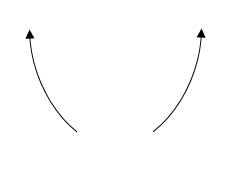
\includegraphics[width=0.3\textwidth]{../Figures/endBehaviorPositiveEvenB.png} \end{center}\begin{tabular}{|c|c|} 
\hline 
 & \tabularnewline 
 \textbf{A.} 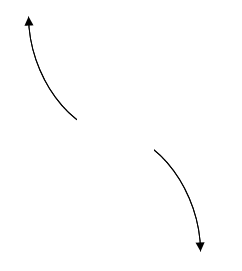
\includegraphics[width=0.3\textwidth]{../Figures/endBehaviorNegativeOddB.png} & \textbf{B.} 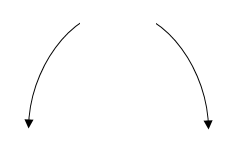
\includegraphics[width=0.3\textwidth]{../Figures/endBehaviorNegativeEvenB.png} \tabularnewline 
\hline 
 & \tabularnewline 
 \textbf{C.} 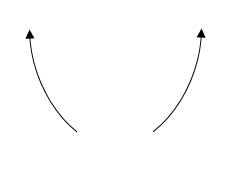
\includegraphics[width=0.3\textwidth]{../Figures/endBehaviorPositiveEvenB.png} & \textbf{D.} 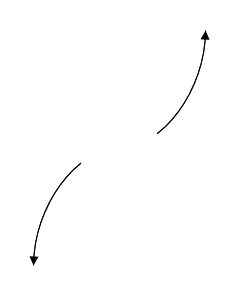
\includegraphics[width=0.3\textwidth]{../Figures/endBehaviorPositiveOddB.png} \tabularnewline 
\hline 
 E. None of the figures above. & \tabularnewline 
\hline 
 \end{tabular} 
 
\textbf{General Comments:} Remember that end behavior is determined by the leading coefficient AND whether the \textbf{sum} of the multiplicities is positive or negative.

-----------------------------------------------

27. Which of the following equations \textit{could} be of the graph presented below?
\begin{center} 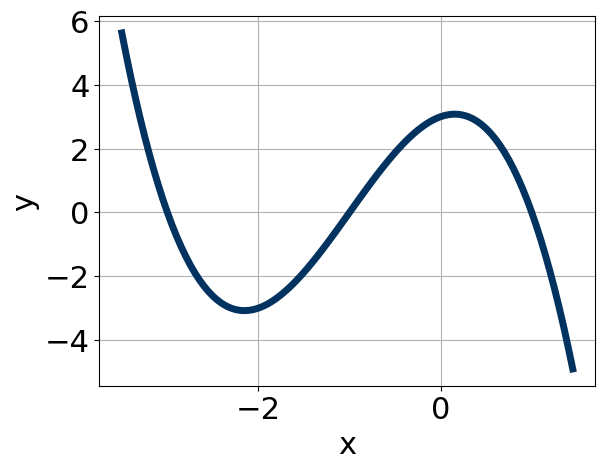
\includegraphics[width=0.3\textwidth]{../Figures/polyGraphToFunctionB.png} \end{center} 

The solution is $ -14(x + 2)^{7} (x - 3)^{11} (x + 3)^{9} $ 

\begin{enumerate}[label=\Alph*.] 
\item $ 13(x + 2)^{11} (x - 3)^{5} (x + 3)^{7} $ 

 This corresponds to the leading coefficient being the opposite value than it should be. 
\item $ -14(x + 2)^{7} (x - 3)^{11} (x + 3)^{9} $ 

 * This is the correct option. 
\item $ -8(x + 2)^{10} (x - 3)^{9} (x + 3)^{11} $ 

 The factor $-2$ should have been an odd power. 
\item $ -12(x + 2)^{8} (x - 3)^{10} (x + 3)^{9} $ 

 The factors $-2$ and $3$ have have been odd power. 
\item $ 5(x + 2)^{10} (x - 3)^{7} (x + 3)^{7} $ 

 The factor $(x + 2)$ should have an odd power and the leading coefficient should be the opposite sign. 
\end{enumerate} 
 
General Comments: Draw the x-axis to determine which zeros are touching (and so have even multiplicity) or cross (and have odd multiplicity).

-----------------------------------------------

28. Construct the lowest-degree polynomial given the zeros below. Then, choose the intervals that contain the coefficients of the polynomial in the form $ax^3+bx^2+cx+d$.
$$ \frac{4}{3}, -2, \text{ and } \frac{-2}{3} $$ 
The solution is $ 9x^{3} +12 x^{2} -20 x -16 $ 

\begin{enumerate}[label=\Alph*.] 
\item $ a \in [4, 13], b \in [35, 39], c \in [43, 46], \text{ and } d \in [13, 26] $ 

 $9x^{3} +36 x^{2} +44 x + 16$, which corresponds to multiplying out $(3x + 3)(x -1)(3x -3)$. 
\item $ a \in [4, 13], b \in [-7, 6], c \in [-32, -23], \text{ and } d \in [-17, -5] $ 

 $9x^{3} -28 x -16$, which corresponds to multiplying out $(3x + 3)(x + 1)(3x -3)$. 
\item $ a \in [4, 13], b \in [4, 14], c \in [-26, -18], \text{ and } d \in [13, 26] $ 

 $9x^{3} +12 x^{2} -20 x + 16$, which corresponds to multiplying everything correctly except the constant term. 
\item $ a \in [4, 13], b \in [-13, -7], c \in [-26, -18], \text{ and } d \in [13, 26] $ 

 $9x^{3} -12 x^{2} -20 x + 16$, which corresponds to multiplying out $(3x + 4)(x -2)(3x -2)$. 
\item $ a \in [4, 13], b \in [4, 14], c \in [-26, -18], \text{ and } d \in [-17, -5] $ 

 * $9x^{3} +12 x^{2} -20 x -16$, which is the correct option. 
\end{enumerate} 
 
General Comments: To construct the lowest-degree polynomial, you want to multiply out $(3x -4)(x + 2)(3x + 2)$

-----------------------------------------------

29. Construct the lowest-degree polynomial given the zeros below. Then, choose the intervals that contain the coefficients of the polynomial in the form $x^3+bx^2+cx+d$.
$$ 2 + 4i \text{ and } -3 $$ 
The solution is $ x^{3} -1 x^{2} +8 x + 60 $ 

\begin{enumerate}[label=\Alph*.] 
\item $ b \in [0.76, 3.05], c \in [7.39, 9.98], \text{ and } d \in [-63, -57] $ 

 $x^{3} + x^{2} +8 x -60$, which corresponds to multiplying out $(x-(2 + 4i))(x-(2 - 4i))(x -3)$. 
\item $ b \in [0.76, 3.05], c \in [0.43, 1.11], \text{ and } d \in [-7, -1] $ 

 $x^{3} + x^{2} +x -6$, which corresponds to multiplying out $(x -2)(x + 3)$. 
\item $ b \in [-2.67, 0.41], c \in [7.39, 9.98], \text{ and } d \in [59, 65] $ 

 * $x^{3} -1 x^{2} +8 x + 60$, which is the correct option. 
\item $ b \in [0.76, 3.05], c \in [-2.3, -0.94], \text{ and } d \in [-15, -9] $ 

 $x^{3} + x^{2} -x -12$, which corresponds to multiplying out $(x -4)(x + 3)$. 
\item $ \text{None of the above.} $ 

 This corresponds to making an unanticipated error or not understanding how to use nonreal complex numbers to create the lowest-degree polynomial. If you chose this and are not sure what you did wrong, please contact the coordinator for help. 
\end{enumerate} 
 
General Comments: Remember that the conjugate of $a+bi$ is $a-bi$. Since these zeros always come in pairs, we need to multiply out $(x-(2 + 4i))(x-(2 - 4i))(x-(-3))$.

-----------------------------------------------

30. Describe the zero behavior of the zero $x = -6$ of the polynomial below.
$$ f(x) = -2(x - 6)^{4}(x + 6)^{7}(x - 9)^{3}(x + 9)^{5} $$ 

 
 The solution is  
 \begin{center} 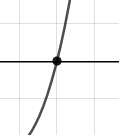
\includegraphics[width=0.3\textwidth]{../Figures/zeroBehaviorPositiveOddB.png} \end{center}\begin{tabular}{|c|c|} 
\hline 
 & \tabularnewline 
 \textbf{A.} 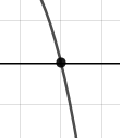
\includegraphics[width=0.3\textwidth]{../Figures/zeroBehaviorNegativeOddB.png} & \textbf{B.} 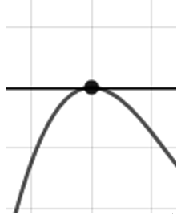
\includegraphics[width=0.3\textwidth]{../Figures/zeroBehaviorNegativeEvenB.png} \tabularnewline 
\hline 
 & \tabularnewline 
 \textbf{C.} 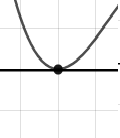
\includegraphics[width=0.3\textwidth]{../Figures/zeroBehaviorPositiveEvenB.png} & \textbf{D.} 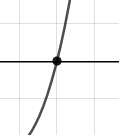
\includegraphics[width=0.3\textwidth]{../Figures/zeroBehaviorPositiveOddB.png} \tabularnewline 
\hline 
 E. None of the figures above. & \tabularnewline 
\hline 
 \end{tabular} 
 
\textbf{General Comments:} You will need to sketch the entire graph, then zoom in on the zero the question asks about.

-----------------------------------------------


\end{document}

